\documentclass{SMR}
%graphics
\graphicspath{ {/Where/you/keep/your/graphics} }  % <- UPDATE THE PATH

%who and where
\smrtitle{SMR.cls}
\smrauthor{Marcin Pietryszwski}
\smraffiliation{Edinburgh University}

\begin{document}

\section{Section One - comment out if not needed} %section title comes here,
                                                  %comment out if there are
                                                  %no sections in the article  
\vspace*{1.0cm}

Here is some text to be formatted followed by a figure of
a Klein Bottle as an example of how graphics are formatted
in this template   

\begin{figure}[h]
\caption{Klein Bottle} %EDIT CAPTION
\centering
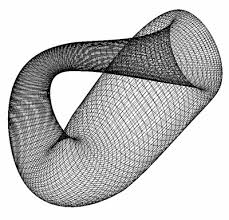
\includegraphics[width=0.5\textwidth]{klein.jpg}
\end{figure}

Here is some text following a figure with a footnote added
to it \footnote{I am a footnote}. Here is an \emph{emphasized text}
followed by \textbf{bold text} which can be used for
\textbf{[Referencing]}

\pagebreak

\subsection{A Subsection} %subsections

Subsections are numbered per section.

\section{A New Section}

This section has its own subsection.

\subsection{Another subsection}

Like this one.

You will find the bibliography on the next page.
\vfill\pagebreak

%a separate section for bibliography

\section*{Bibliography}

\end{document}
